
Асинхронность компонента хранения достигается за счет использования объектов-обещаний (Promise), по своей природе являющихся указателями на длительную асинхронную операцию. 

Механизм работы объекта обещания изображен на рисунке \ref{fig:theory:promise} и состоит в следующем:

\begin{enumerate}[label=\arabic*.]
\item{Объект <<потребитель>> вызывает <<сервис>> с целью получить некоторые данные либо вызвать удаленный API, ответ от которого может занять неопределенное время.}
\item{Сервис создает объект типа \texttt{Promise<T>}, где \texttt{T} -- тип ожидаемого потребителем значения (может быть \texttt{void}).}
\item{Конструктор типа \texttt{Promise<T>} принимает в качестве аргумента функцию сигнатуры \texttt{(resolve: (T) => void, reject: (any) => void) => void}. Внутри данной функции, сервис
обращается к долгоработающему API (<<сторонний сервис>>) -- это может быть unmanaged-код, управляемый системой сигналов или другой сервис. Единственным требованием к долгоработающему API
является наличие некоторго механзма оповещения о завершении операции. Например, вызов callback-функции или некоторого сигнала.)}
\item{После начала длительной операции и возвращения объекта типа \texttt{Pro- mise<T>}, <<Потребитель>> продолжает свою работу, ожидая ответа от результата длительного вызова. Данные
действия производятся синхронно старту длительной операции. Объект потребитель может делать другие долгие вызовы, обращаться к другим сервисам и т.д.}
\item{После того как все синхронные операции завершатся, поток, обрабатывающий поведение объекта потребителя завершит работать и выйдет за пределы области пользовательского кода,
виртуальная машина языка JavaScript начнет ожидать очередного события в очереди. Рано или поздно, от <<стороннего сервиса>> придет ответ и будет вызвана callback-функция либо сработает
сигнал, который будет воспринят <<сервисом>>.}
\item{Контроль будет передан callback-функции <<сервиса>>, которая либо вызовет функцию \texttt{resolve: (T) => void} с некоторым результатом операции в качестве аргумента,
сигнализируя объекту-обещанию о том, что долгоработающая операция завершилась успешно и были получены данные типа T, либо функцию \texttt{reject: (any) => void}, сигнализирующая
об ошибке. Во втором случае, может быть передан описатель ошибки любого типа и <<потребитель>> может обработать ее соответствующим образом.}
\item{Вызов \texttt{resolve} или \texttt{reject} вызывает обработчики, зарегистрированные объектом <<потребитель>>, тем самым возобновляя процесс выполнения программы.}
\end{enumerate}

\begin{figure}[ht]
\centering
  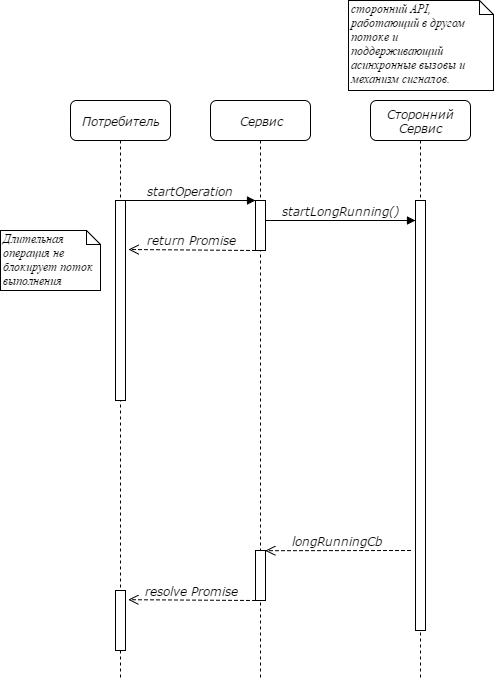
\includegraphics[scale=0.71]{promise.png}
  \caption{Диаграмма последовательности работы Promise-объекта}
  \label{fig:theory:promise}
\end{figure}

Техника создания и использования объектов обещаний приведена на листинге ниже на примере длительной операции чтения содержимого удаленного ресурса, который был сохранен в
файл на жестком диске и помещение этого содержимого в \texttt{Blob}-объект:
\begin{lstlisting}[language=TypeScript, showstringspaces=false, label=lst:dev:framelements4]

private static buildImageBlob(src: string): Promise<HTMLImageElement> {
    // Create promise and pass it a (resolve, reject) => void
    return new Promise<HTMLImageElement>((resolve, reject) => {
        // Start a long running operation with a callback argument
        fs.readFile(this.getResourcePath(src), (err: any, contents: Buffer) => {

            // After the long-running operation is done, check the status.
            // Reject in case of error
            if (err) reject(err);

            // Transform the result and resolve the promise in case of success.
            let dataBlob = new Blob([contents], { type: 'image/png' });
            let img = new Image()
            img.src = URL.createObjectURL(dataBlob);
            resolve(img);
        });
    });
}

public static getImageResource(src: string): Promise<HTMLImageElement> {
    return new Promise<HTMLImageElement>((resolve, reject) => {
        if (!this.doesResourceExist(src)) {
            this.prefetchImage(src).then((resourcePath) => {
                this.buildImageBlob(src).then(resolve);
            });
        } else {
            this.buildImageBlob(src).then(resolve);
        }
    });
}
\end{lstlisting}

Как показано на листинге выше, операции можно объединять в цепочки и вызывать одну за другой после завершения, однако не блокируя при этом поток выполнения. Такой подход,
когда одна операция возвращает обещание на результат, а другая возвращает обещание на обработанный результат непосредственно после получения результата первой (и так далее),
получил название <<неблокирующее программирование>> и напоминает по своей сути реактивное программирование. Системы, которые построены таким образом, определяют очередь
операций и порядок их завершения в основном (управляющем) потоке, тогда как сами операции выполняются в отдельных потоках или же совершенно другими процессорами в целом.
Следует отметить, однако, что виртуальная машина языка JavaScript выполняется в один поток и, соответственно, выполняет данную очередь в один поток. Виртуальная машина
решает о том, какая асинхронная операция будет выполняться следующей либо выполняет ее обработку только в том случае, если пользовательский код достиг последней своей
инструкции и вышел в область управления виртуальной машины. Только в этом случае, язык может начать прослушивать сигналы и обрабатывать приходящие извне события. Это
означает, что несмотря на видимую сложность организации подобных систем, где обновление внутреннего состояния происходят асинхронно и каскадами, она полностью
потокобезопасна.
Использование механизма Promise-обещаний позволяет избежать одного из наиболее серьезных антипаттернов программирования в среде node.js -- так
называемый \textit{callback hell} -- антипаттерн, возникающий в системах, где используется слишком много асинхронных вызовов и их обработка производится
посредством вызова callback-функций. Поддержка и расширение очереди команд в такой системе становится сложнее и сложнее с каждой добавленной callback-функцией 
не только из-за добавленной логики, но и потому что для цикличных вызовов очень сложно извлечь общую логику с целью использовать цикл. Механизм Promise-объектов
позволяет лучше упорядочить очередь асинхронных вызовов а также реализует множество методов, позволяющих комбинировать Promise-объекты. Так, например,
библиотека \texttt{\$q} реализует методы, позволяющие получить Promise-объект, комбинирующий коллекцию Promise-объектов коллекции завершили выполнение, либо когда
завершил выполнение один из них. Библиотека \texttt{\$q} используется в процессе модульного тестирования всего компонента \texttt{Persistance}, потому как данный модуль
тесно связан с модулем \texttt{fs} из стандартной библиотеки node.js, реализующей асинхронный доступ к файловой системе компьютера и интерфейсы используемых компонентов
и их mock-реализаций должны совпадать.

